\documentclass[11pt]{article}
\usepackage[top=0.7in,bottom=0.75in,left=0.85in,right=0.85in]{geometry}
\usepackage{graphicx}
\usepackage{amsmath, amssymb}
\usepackage{microtype}
\usepackage[hidelinks]{hyperref}
\usepackage{caption}
\captionsetup{font=small,labelfont=bf,skip=4pt}
\usepackage{titlesec}
\titlespacing*{\section}{0pt}{6pt}{2pt}
\titlespacing*{\subsection}{0pt}{4pt}{1pt}
\titleformat{\section}{\normalfont\large\bfseries}{\thesection}{0.6em}{}
\titleformat{\subsection}{\normalfont\bfseries}{\thesubsection}{0.5em}{}
\setlength{\parskip}{2pt}
\setlength{\parindent}{1em}
\frenchspacing

\title{\vspace{-2em}Inverse Transition Learning from Expert Demonstrations:\\
\large Reproduction and a Joint Reward--Dynamics Extension}
\author{Agna Chan \\ \small Columbia University \quad Advisor: Prof.\ Bianca Dumitrascu}
\date{\small May 2026}

\begin{document}
\maketitle
\vspace{-2em}

\section{Question}

In standard reinforcement learning we know the transition dynamics $T$ of a Markov decision process and want to compute an optimal policy $\pi^{*}$. Many real settings invert that assumption. In an intensive care unit, for example, the reward (patient outcome) is observable but the dynamics of how a patient responds to a particular dose are not. What we observe is a batch of clinician decisions that are close to optimal but not exactly optimal. The question this semester has been: given the reward $R$ and a batch of $\varepsilon$-optimal expert transitions $D = \{(s, a, s')\}$, can we recover the dynamics $T^{*}$ in a way that respects the optimality information in the actions, rather than throwing it away as a maximum-likelihood estimate over counts does?

The paper that frames this problem is \emph{Inverse Transition Learning} \cite{benac2024itl}. The method I have been studying and reproducing is the convex quadratic program in their Algorithm~1.

\section{Method and tools}

An action $a$ is $\varepsilon$-optimal at state $s$ under dynamics $T$ when $\max_{a'} Q^{*}(s, a'; T) - Q^{*}(s, a; T) \le \varepsilon$. Observing the expert choose $a$ at $s$ therefore yields an inequality on $Q^{*}$. Writing the policy-evaluation inverse $v^{\pi} = (I - \gamma P^{\pi})^{-1} r^{\pi}$ and substituting the Laplace-smoothed MLE $T^{\mathrm{MLE}}$ inside the inverse \emph{linearizes} the constraint in $T$. The resulting program is
\begin{equation*}
\min_{T} \;\; \tfrac{1}{2}\sum_{s,a,s'} N_{s,a,s'} \bigl(T_{s,a,s'} - T^{\mathrm{MLE}}_{s,a,s'}\bigr)^{2}
\quad \text{s.t.} \quad
\text{$\varepsilon$-ball constraints on $(s,a) \in D$, simplex on $T$.}
\end{equation*}
The solver alternates between a policy estimate $\hat\pi$ (uniform over observed actions at observed states; uniform over actions elsewhere, per Algorithm 1, line 3) and the QP above, terminating when the $\varepsilon$-ball property holds at every observed state. The convex pieces are standard tabular RL machinery from \cite[Ch.~10]{krause2025pai}: Bellman optimality, policy-induced matrices, and the linear policy-evaluation system. The Laplace-smoothed MLE corresponds to a Dirichlet posterior mean from the same textbook's Chapter~11 on Bayesian model-based RL. The implementation uses CVXPY \cite{diamond2016cvxpy} with an OSQP--SCS--CLARABEL fallback chain.

\section{Simulation: coverage sweep on Gridworld}

I reproduced the paper's central empirical claim (their Figure~2) on a 5$\times$5 Gridworld with soft walls at five tiles (penalty $-5$), slip probability $0.2$, $\gamma = 0.95$, and $\varepsilon = 5.0$. The expert was 40\% stochastic, meaning at 40\% of states the expert mixes uniformly over the $\varepsilon$-ball rather than acting greedily. \emph{Coverage} is the fraction of states that appear in $D$; for each observed $(s,a)$ I sampled 10 transitions. I compared two estimators of $T$: the Laplace-smoothed MLE and ITL.

\begin{figure}[h]
\centering
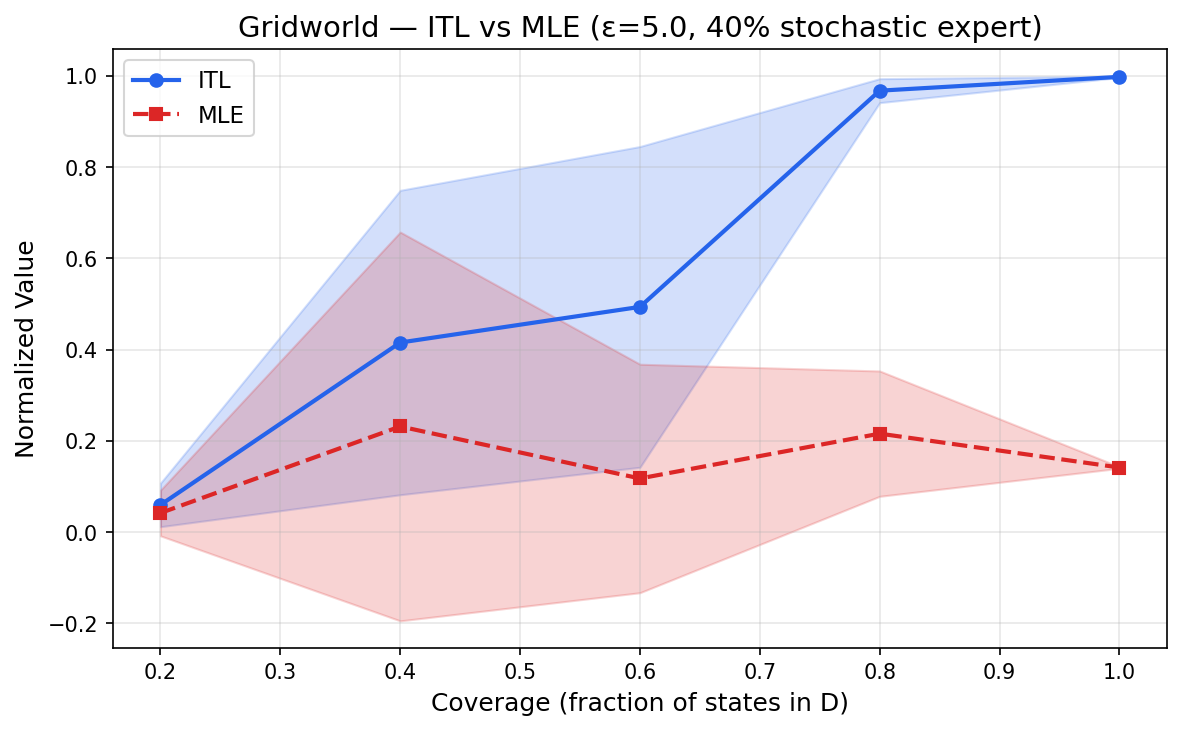
\includegraphics[width=0.58\textwidth]{gridworld_nv.png}
\caption{Normalized Value $V^{\pi^{*}(\hat T)}(s_0; T^{*}) / V^{\pi^{*}(T^{*})}(s_0; T^{*})$ vs.\ coverage on Gridworld. ITL plateaus near $1.0$ at full coverage and dominates MLE everywhere. Shaded bands: $\pm 1$ std.\ across seeds.}
\label{fig:nv}
\end{figure}

At full coverage, ITL achieves Normalized Value $0.998 \pm 0.001$ versus MLE's $0.142 \pm 0.002$, with $0.00$ versus $7.20$ constraint violations and $\varepsilon$-matching $1.000$ versus $0.712$ (averages over 5 seeds). MLE's argmax under-counts visited next-state cells when the expert is occasionally stochastic, so the greedy policy under $\hat T_{\mathrm{MLE}}$ walks into soft walls. ITL avoids this by enforcing that the expert's observed choices remain $\varepsilon$-optimal under $\hat T$. The qualitative shape matches the paper's Figure~2; the absolute scale runs roughly $1.5\times$ larger than Table~4, almost certainly because the published soft-wall layout is not reported in detail, so my environment is somewhat less aversive. The structural pattern (ITL $\ge$ MLE on every metric, $\varepsilon$-matching $\to 1.0$ for ITL at full coverage as predicted by Theorem~1) holds on both Gridworld and a separate RandomWorld benchmark.

\section{Open question: joint reward and dynamics recovery}

The paper assumes $R$ is known. In MIMIC-IV that assumption is fragile: the survival proxy reward ($\pm 15$ for discharge or mortality, after \cite{komorowski2018aic}) is hand-engineered. The thesis extension I have been prototyping, which the paper itself names as future work, is to lift $R$ into a decision variable parameterized as $R(s,a) = \Phi(s,a)^{\top} w$ and solve for $(T, w)$ jointly. The $\varepsilon$-ball constraint becomes
\begin{equation*}
\bigl(\Phi(s,a) - \Phi(s,a')\bigr)^{\top} w + \gamma\,(T_{s,a} - T_{s,a'})^{\top} v_{\mathrm{lin}} \;\ge\; \varepsilon.
\end{equation*}
This is bilinear in $(T, w)$ once $v_{\mathrm{lin}}$ is treated as a function of $w$, but each step of an alternation (hold $w$, solve for $T$; hold $T$, solve for $w$) is a convex QP. An L1 penalty on $w$ plus an anchor at one $(s,a)$ pin the additive ambiguity. Inspired by maximum-entropy IRL \cite{ziebart2008maxent}, but distinct from it because the dynamics are not assumed known.

A smoke test on the 3-state corridor with state-only one-hot features and the goal reward as anchor terminates at a fixed point in two outer iterations. The recovered policy matches the true optimal policy exactly. Transition MSE is $0.233$, comparable to ITL alone with known $R$ ($0.237$) and below the MLE baseline ($0.282$). The reward weights are recovered up to the L1 sparsity that the regularizer enforces on the small near-zero true weights, which is the expected identifiability behavior of one-hot state-only features. Stress tests on Gridworld and a baseline against MaxEnt-IRL with a separately estimated $T$ are the next steps before the May 31 thesis draft.

\paragraph{Code and reproducibility.} The full reproduction codebase (Python 3.10, CVXPY, MIT-licensed) is at \url{https://github.com/REPLACE-ME/itl-reproduction}, with inline cross-references between paper equations, textbook chapters, and source lines. A Colab that re-runs the corridor sanity check, the Gridworld coverage sweep at a reduced seed count, and the ITL+IRL smoke test that produced the numbers in Section~4 is at \url{https://colab.research.google.com/REPLACE-ME}.

{\scriptsize
\renewcommand{\section}[2]{}%
\begin{thebibliography}{9}
\setlength{\itemsep}{0pt}
\setlength{\parsep}{0pt}
\bibitem{benac2024itl} Benac, L., et al.\ (2024). Inverse Transition Learning: Learning Dynamics from Demonstrations. \emph{AAAI 2025} (preprint).
\bibitem{krause2025pai} Krause, A., and H\"ubotter, J.\ (2025). \emph{Probabilistic Artificial Intelligence}. Cambridge Univ.\ Press. Ch.\ 10--12.
\bibitem{ziebart2008maxent} Ziebart, B.~D., Maas, A., Bagnell, J.~A., and Dey, A.~K.\ (2008). Maximum Entropy Inverse Reinforcement Learning. \emph{Proc.\ AAAI}.
\bibitem{komorowski2018aic} Komorowski, M., Celi, L.~A., Badawi, O., Gordon, A.~C., and Faisal, A.~A.\ (2018). The Artificial Intelligence Clinician learns optimal treatment strategies for sepsis in intensive care. \emph{Nature Medicine} 24, 1716--1720.
\bibitem{diamond2016cvxpy} Diamond, S., and Boyd, S.\ (2016). CVXPY: A Python-Embedded Modeling Language for Convex Optimization. \emph{JMLR} 17(83), 1--5.
\end{thebibliography}}

\end{document}
